本节介绍了提供组中工作项间通信的构建块。一些基本的构建块,可以构建自定义算法,而另一些高级别的,则描述了许多内核的常规操作。\par

\hspace*{\fill} \par %插入空行
\textbf{通过栅栏进行同步}

通讯最基本的部分是栅栏功能。栅栏功能有两个目的:\par

首先,栅栏功能可以同步组中工作项的执行。通过同步,工作项可以确保另一个工作项在使用该操作的结果之前完成操作。在另一个工作项使用操作的结果之前,让工作项完成操作。\par

其次,栅栏函数同步每个工作项,并检查内存状态。这种类型的同步操作称为强制内存一致或隔离内存(详见第19章)。内存一致与同步执行一样重要,因为在栅栏前执行的内存操作对栅栏之后执行的其他工作项可见。如果没有内存一致性,工作项中的操作就像森林中倒下的一棵树,其他工作项不一定听得到声音!\par

图9-2显示了在栅栏功能上同步组中的四个工作项。尽管每个工作项的执行时间可能不同,但没有任何工作项可以跨过栅栏执行,直到所有工作项都遇到了栅栏。执行栅栏功能之后,所有工作项就有了一致的内存。\par

\hspace*{\fill} \par %插入空行
图9-2 组中的四个工作项在栅栏功能上的同步
\begin{center}
	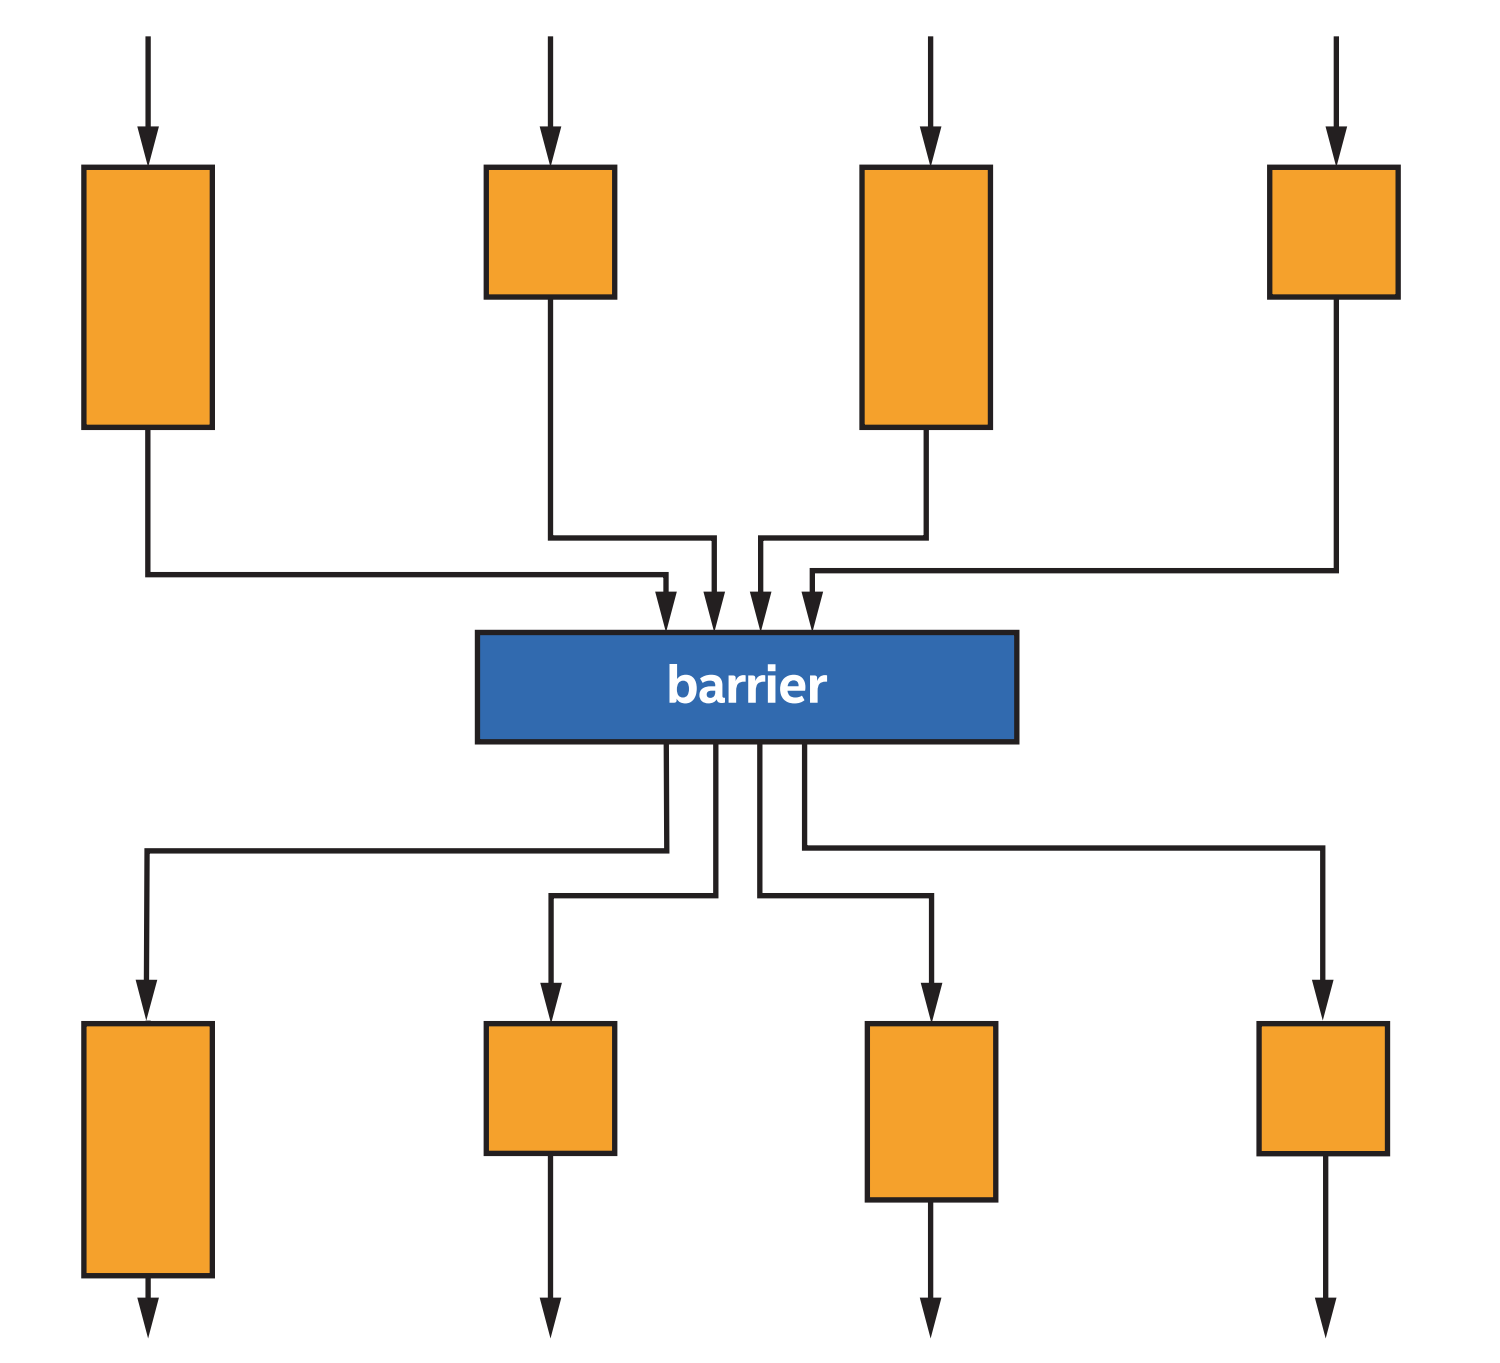
\includegraphics[width=0.6\textwidth]{content/chapter-9/images/3}
\end{center}

\begin{tcolorbox}[colback=blue!5!white,colframe=blue!75!black, title=为什么内存在默认情况下不一致?]
对于许多开发者来说,内存一致性的概念——以及不同的工作项可以看到不同的内存数据——可能感觉非常奇怪。如果默认情况下所有工作项的所有内存都是一致的,不是更容易吗?是的,但实现的代价非常昂贵。允许工作项看到不一致的内存数据,并且只要求程序执行期间定义的点上保证内存一致性,这样加速器硬件价格会更便宜,性能更好。
\end{tcolorbox}

因为栅栏功能同步执行,所以要么组中的所有工作项执行栅栏操作,要么组中没有工作项执行栅栏操作。如果组分支中的某些工作项绕过栅栏功能,则组中的其他工作项可能永远在栅栏处等待!\par

\begin{tcolorbox}[colback=blue!5!white,colframe=blue!75!black, title=集合功能]
当一个功能需要由组中的所有工作项执行时,可以将其称为集合功能,因为操作由工作组执行,不由组中的单个工作项执行。栅栏函数并不是SYCL中唯一可用的集合函数。本章稍后将介绍其他集合功能。
\end{tcolorbox}

\hspace*{\fill} \par %插入空行
\textbf{工作组的本地内存}

工作组栅栏功能可以协调工作组中工作项的通信,但是通信必须通过内存进行。通信可以通过USM或缓冲区进行,但这可能效率低下:需要为通讯开辟专用内存,并需要在工作组之间进行分配。\par

为了简化内核开发,并加速工作组中工作项的通信,SYCL定义了专用于工作组中工作项之间通信的本地内存。\par

\hspace*{\fill} \par %插入空行
图9-3 每个工作组可以访问所有全局内存,但只能访问自己的本地内存
\begin{center}
	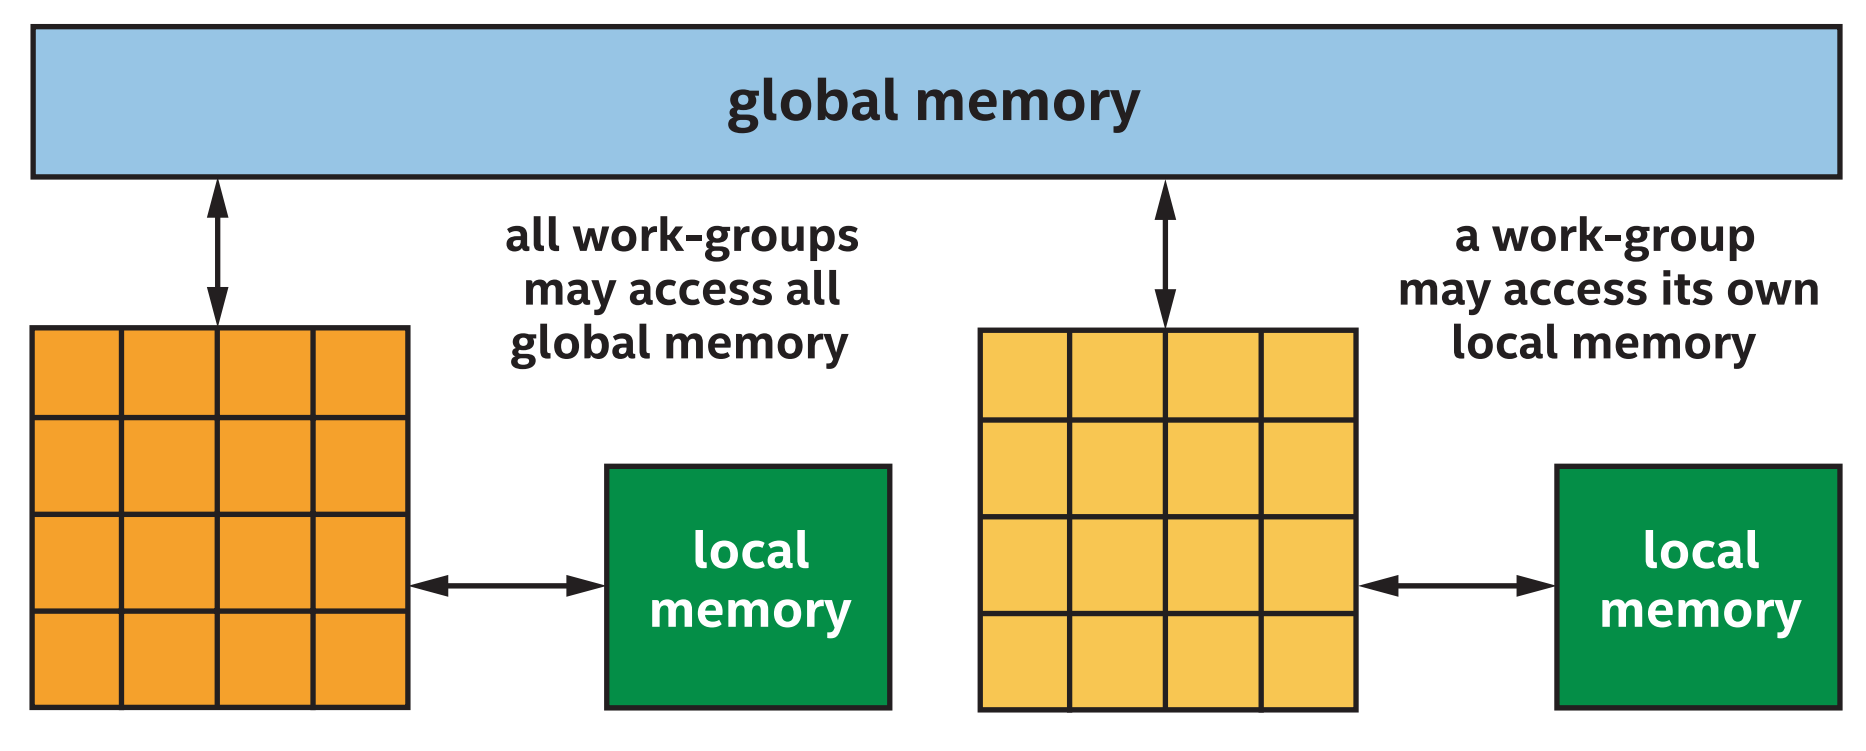
\includegraphics[width=1.\textwidth]{content/chapter-9/images/4}
\end{center}

如图9-3所示,两个工作组可以访问全局内存空间中的USM和缓冲区。每个工作组可以访问自己的本地内存中的变量,但不能访问另一个工作组的本地内存中的变量。\par

当一个工作组开始时,其本地内存的内容未初始化,并且本地内存在工作组执行完毕后不会持续存在。由于这些属性,本地内存只能在工作组执行时作为临时存储使用。\par

对于某些设备,本地内存是一种抽象概念,使用与全局内存相同的内存子系统来实现。设备上使用本地内存,主要是以便通信机制的使用。一些编译器可能会使用内存空间信息进行编译器优化;否则,设备上使用本地内存进行通信,并不会比通过全局内存进行通信的性能更好。\par

对于其他设备,比如:多GPU设备,有专用的本地内存资源。这些设备上,通过本地内存通信比通过全局内存通信性能更好。\par

\begin{tcolorbox}[colback=red!5!white,colframe=red!75!black]
使用本地内存时,工作组内部的通信可以更方便、更快捷!
\end{tcolorbox}

可以使用设备查询info::device::local\_mem\_type来确定加速器是否为本地内存提供了专用资源,或者本地内存是否实现为全局内存。有关查询设备属性的更多信息请参见第12章,有关本地内存如何为CPU、GPU和FPGA实现的更多信息详见第15、16和17章。\par





































